\documentclass{amsart}

\usepackage[T1]{fontenc}
\usepackage[utf8]{inputenc}
\usepackage{amsmath,amssymb}
\usepackage{booktabs}
\usepackage[table]{xcolor}
\usepackage{array}
\usepackage{tikz}

\title{Pebbling Report for Selected Graphs}
\author{}
\date{}

\begin{document}

\maketitle

The table below records the stacking number for each selected graph.
For non-bipartite graphs it also records the clearing number.

\begin{center}
\setlength{\tabcolsep}{10pt}
\renewcommand{\arraystretch}{1.2}
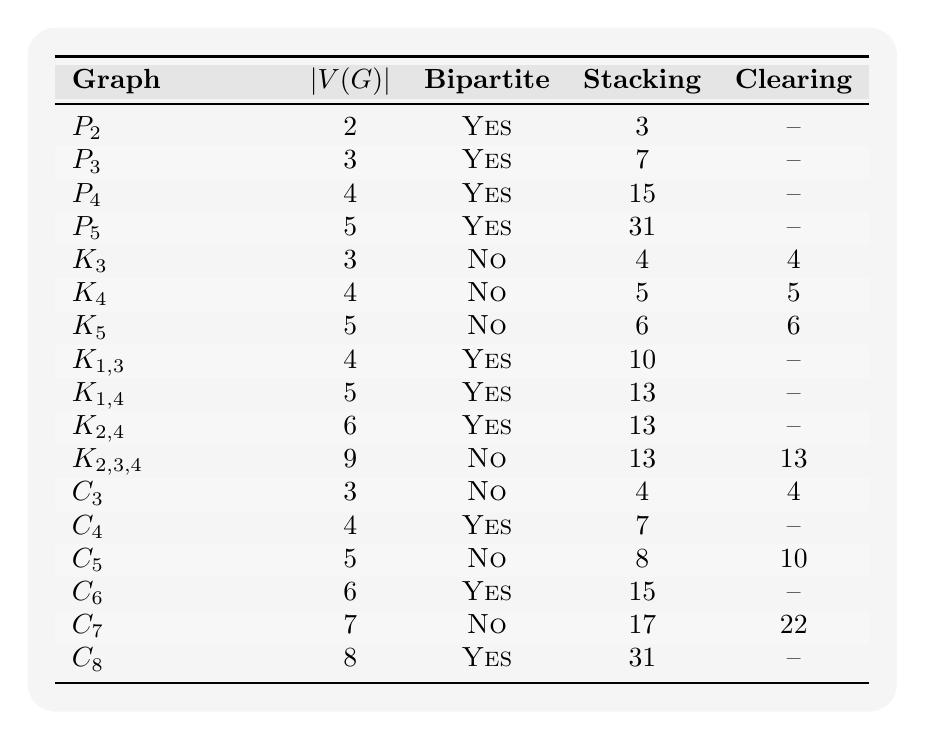
\begin{tikzpicture}
\node[rounded corners=10pt, fill=gray!8, inner sep=10pt] {
\begin{tabular}{>{\raggedright\arraybackslash}p{2.6cm}cccc}
\toprule
\rowcolor{gray!20}
\textbf{Graph} & \textbf{$|V(G)|$} & \textbf{Bipartite} & \textbf{Stacking} & \textbf{Clearing} \\
\midrule
$P_2$ & 2 & \textsc{Yes} & 3 & -- \\
\rowcolor{gray!6} $P_3$ & 3 & \textsc{Yes} & 7 & -- \\
$P_4$ & 4 & \textsc{Yes} & 15 & -- \\
\rowcolor{gray!6} $P_5$ & 5 & \textsc{Yes} & 31 & -- \\
$K_3$ & 3 & \textsc{No} & 4 & 4 \\
\rowcolor{gray!6} $K_4$ & 4 & \textsc{No} & 5 & 5 \\
$K_5$ & 5 & \textsc{No} & 6 & 6 \\
\rowcolor{gray!6} $K_{1,3}$ & 4 & \textsc{Yes} & 10 & -- \\
$K_{1,4}$ & 5 & \textsc{Yes} & 13 & -- \\
\rowcolor{gray!6} $K_{2,4}$ & 6 & \textsc{Yes} & 13 & -- \\
$K_{2,3,4}$ & 9 & \textsc{No} & 13 & 13 \\
\rowcolor{gray!6} $C_3$ & 3 & \textsc{No} & 4 & 4 \\
$C_4$ & 4 & \textsc{Yes} & 7 & -- \\
\rowcolor{gray!6} $C_5$ & 5 & \textsc{No} & 8 & 10 \\
$C_6$ & 6 & \textsc{Yes} & 15 & -- \\
\rowcolor{gray!6} $C_7$ & 7 & \textsc{No} & 17 & 22 \\
$C_8$ & 8 & \textsc{Yes} & 31 & -- \\
\bottomrule
\end{tabular}
};
\end{tikzpicture}
\end{center}

\end{document}
